        \subsection{probability density functions}
\begin{frame}{audio signal description}{probability and occurrence}
	\begin{itemize}
		\item[]	$N$: number of overall observations
		\item[] $N(x_i)$: number of occurrences of symbol $x_i$
	\end{itemize}
	
	\pause
	\begin{itemize}
		\item	relative number of occurrences:
				\begin{equation}
					\hat{p}_i = \frac{N(x_i)}{N}
				\end{equation}
		
		\pause
		\item	probability:
				\begin{equation}
					p_i = \lim\limits_{N\rightarrow\infty} \frac{N(x_i)}{N}
				\end{equation}
	\end{itemize}
    \pause
    \begin{block}{properties}
        \begin{itemize}
            \item[]   $\sum\limits_i p_i = 1$
            \item[]   $0 \leq p_i \leq 1$
        \end{itemize}
    \end{block}
\end{frame}

\begin{frame}{audio signal description}{probability distribution example}
        \vspace{-5mm}
        \begin{itemize}
            \item roll of a die
                \begin{footnotesize}
                \begin{table}
                    \centering
                        \begin{tabular}{lcccccc}
                        \textbf{value} & 1&2&3&4&5&6\\
                        \textbf{p(x)} & \nicefrac{1}{6}& \nicefrac{1}{6}& \nicefrac{1}{6}& \nicefrac{1}{6}& \nicefrac{1}{6}& \nicefrac{1}{6}
                        \end{tabular}
                \end{table}
                \end{footnotesize}
            \pause
            \item probability distribution for the roll of two dice?
            \pause
            \begin{footnotesize}
            \begin{table}
                \centering
                    \begin{tabular}{lccccccccccc}
                    \textbf{value} & 2&3&4&5&6&7&8&9&10&11&12\\
                    \textbf{p(x)} & \nicefrac{1}{36}& \nicefrac{1}{18}& \nicefrac{1}{12}& \nicefrac{1}{9}& \nicefrac{5}{36}& \nicefrac{1}{6}& \nicefrac{5}{36}& \nicefrac{1}{9}& \nicefrac{1}{12}& \nicefrac{1}{18}& \nicefrac{1}{36}
                    \end{tabular}
            \end{table}
            \end{footnotesize}
            \begin{figure}
                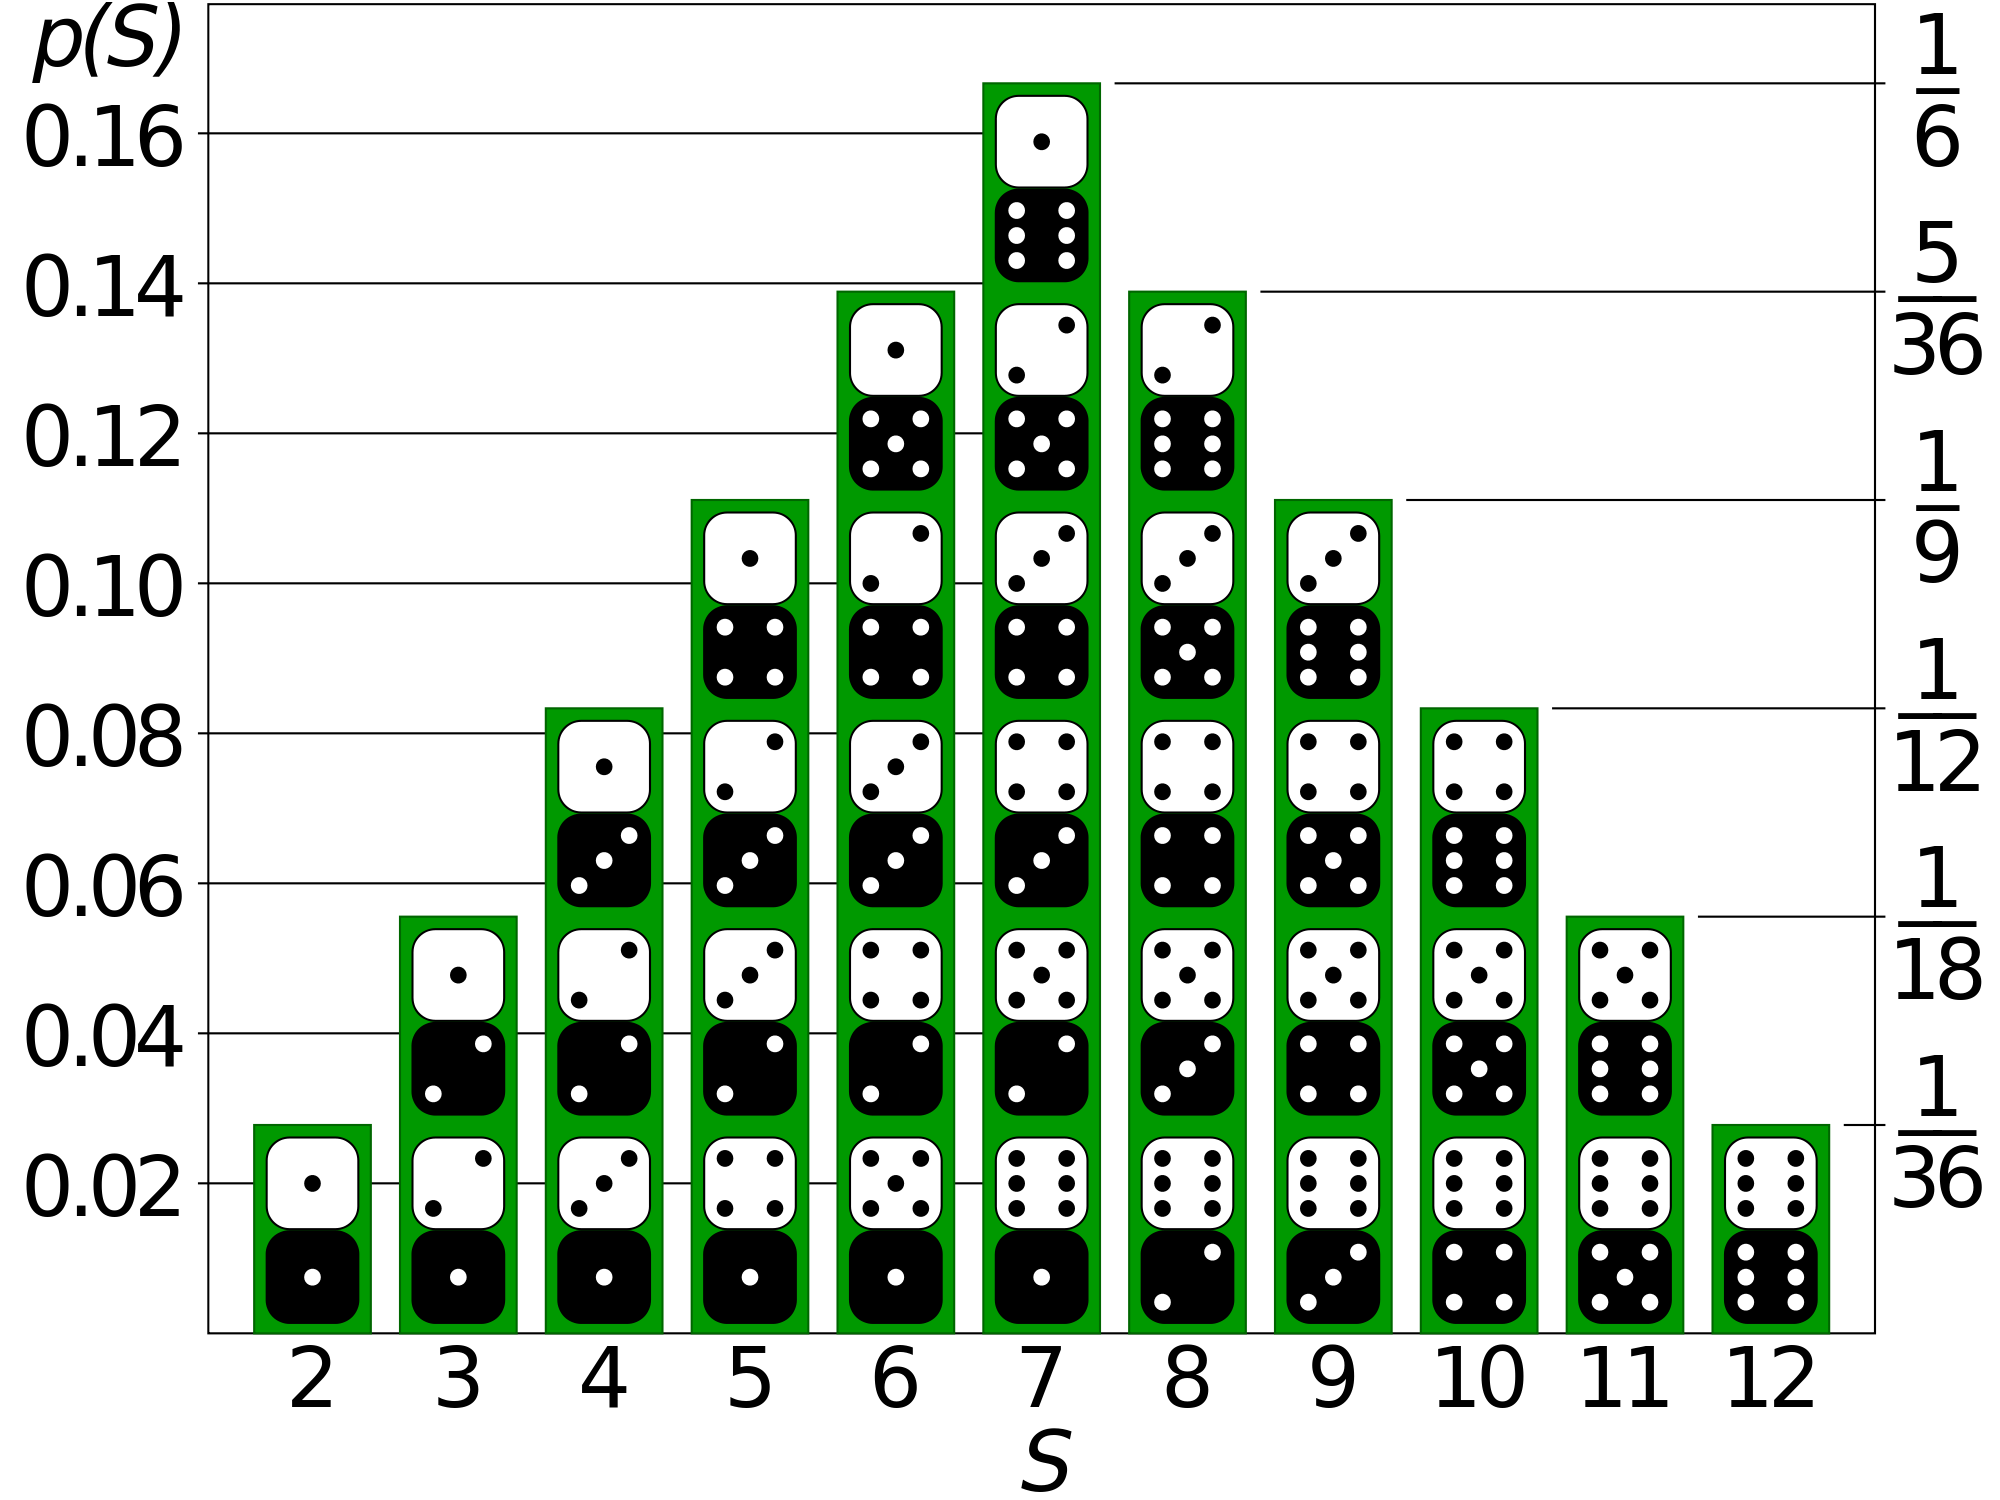
\includegraphics[scale=.08]{graph/diceprobdist}
            \end{figure}
        \end{itemize}
\end{frame}


\begin{frame}{audio signal description}{continuous probability density distribution}
	$i\rightarrow$ continuous $\Rightarrow$ \textbf{PDF} 

	\pause
	\begin{eqnarray}
		\int\limits_{-\infty}^{\infty} p_X(x)dx = 1\\
		0 \leq p_X(x)
	\end{eqnarray}		

	\pause
	Probability of $x$ being a value smaller than or equal $x_c$
				\begin{equation}
					\int\limits_{-\infty}^{x_c} p_X(x)dx
				\end{equation}		
\end{frame}	
	
\begin{frame}{audio signal description}{example PDF: Gaussian}
	\begin{equation} \label{gaussverteilung}
		p_X(x)= \frac{1}{\sqrt{2\pi}\sigma_X}e^{-\frac{(x-\mu_X)^2}{2\sigma_X^2}}
	\end{equation}
	\begin{figure}
		\centering
			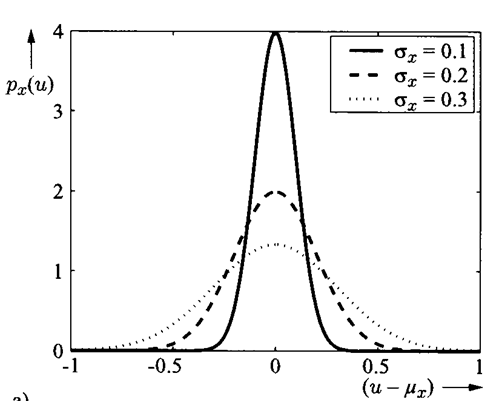
\includegraphics[scale=.5]{graph/gaussdist}
	\end{figure}
\end{frame}	

\begin{frame}{audio signal description}{example PDF: Exponential}
	\begin{equation}
		p_X(x)= \left\lbrace  \begin{array}{ll}
		  \frac{1}{\sigma_X}e^{-\frac{x}{\sigma_X}} & x >0 \\
		  0 & \textrm{else} 
	\end{array}\right.
	\end{equation}
    \begin{figure}
		\centering
			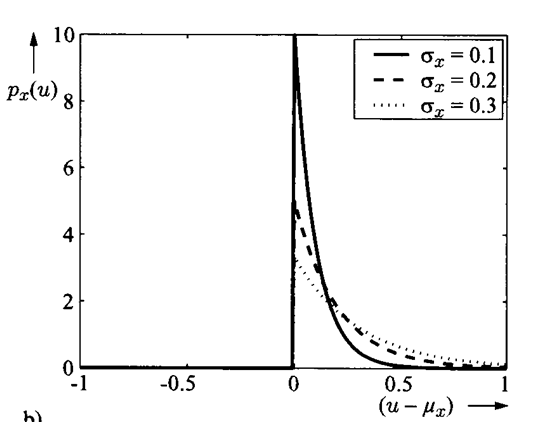
\includegraphics[scale=.5]{graph/expdist}
	\end{figure}
\end{frame}	
	
\begin{frame}{audio signal description}{example PDF: Laplace (2-sided exp)}
	\begin{equation}
		p_X(x)= \frac{1}{\sqrt{2}\sigma_X}e^{-\sqrt{2}\frac{\mid x-\mu_X\mid}{\sigma_X}}
	\end{equation}
	\begin{figure}
		\centering
			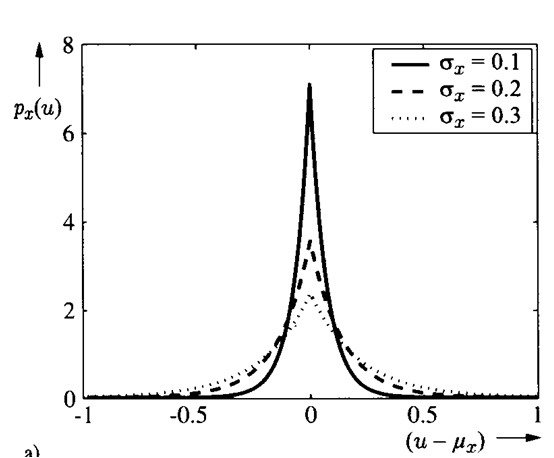
\includegraphics[scale=.5]{graph/laplacedist}
	\end{figure}
\end{frame}	

\begin{frame}{audio signal description}{measured RDF}
	\begin{figure}
		\centering
            \only<1>{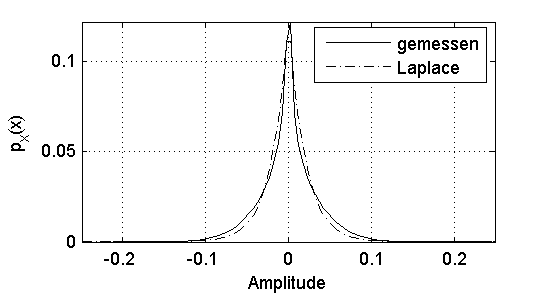
\includegraphics[scale=1.]{graph/Lerch14-9}}
            \only<2>{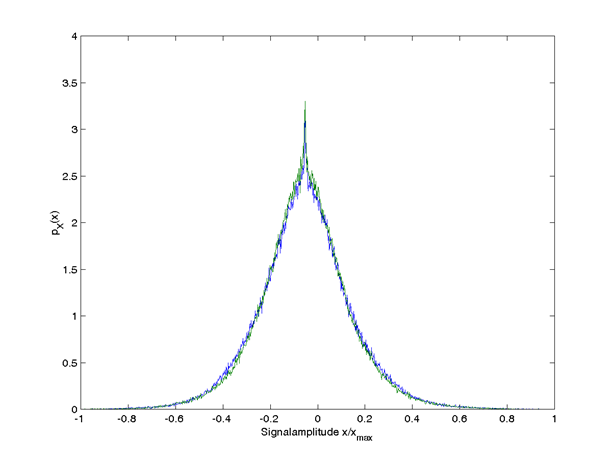
\includegraphics[scale=.5]{graph/pdf}}
	\end{figure}
\end{frame}	
	
\begin{frame}{audio signal description}{PDFs of generated signals 1/2}
	\vspace{-15mm}
	\begin{columns}
		\column{5cm}
		Draw the following PDFs:
		
		\column{4cm}
		%\hspace{5mm}
		\begin{flushright}
			 
\includegraphics[scale=.08]{Graph/question-mark}
		\end{flushright}
	\end{columns}
	\pause
	\begin{itemize}
		\item	white noise (uniform)
		\item	white noise (Gaussian)
		\item	DC
		\item	square
		\item	sinusoidal
		\item	sawtooth
	\end{itemize}
\end{frame}	
	
\begin{frame}{audio signal description}{distributions of generated signals 2/2}
	\begin{figure}
		\centering
			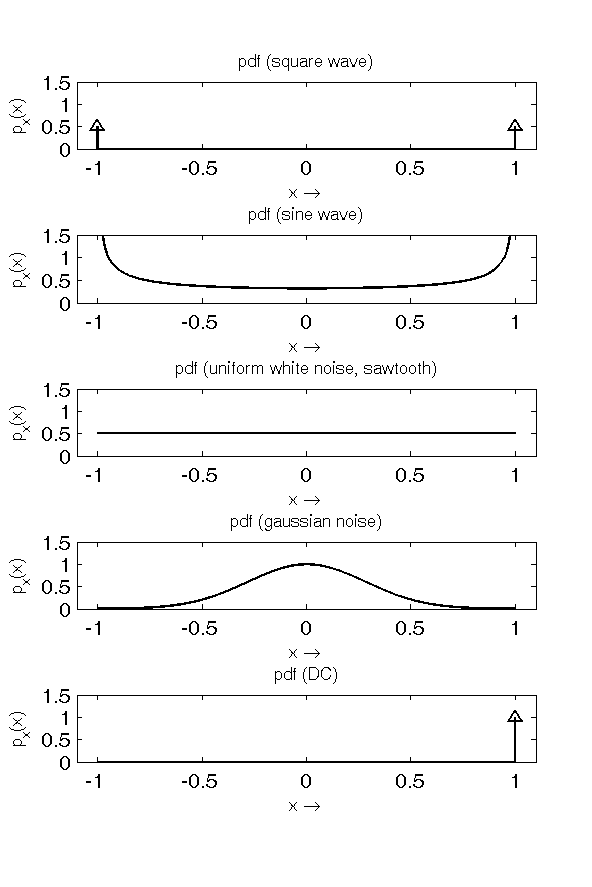
\includegraphics[scale=.5]{graph/pdfs}
	\end{figure}
\end{frame}	
	
\begin{frame}{audio signal description}{expected value 1/3}
	Example: average grade, five students, grades: 1, 2, 1, 3, 5

	\uncover<1->{
	\begin{equation}
		\hat{\mu}_X = \frac{1+2+1+3+5}{5} = 2.4
	\end{equation}
	}
	\uncover<2->{
		\begin{table}[!hbt]
			\begin{center}
			\begin{footnotesize}
				\begin{tabular}{lcr}
				\hline
					\textbf{Grade} & \textbf{\# occurrences} & \textbf{relative frequency} \\
				\hline
					1	&	2	& $2/5$	\\
					2	&	1	& $1/5$	\\
					3	&	1	& $1/5$	\\
					4	&	0	& $0/5$	\\
					5	&	1	& $1/5$	\\
				\hline
				\end{tabular}  
			\end{footnotesize}
			\end{center}
		\end{table}
	}
\end{frame}		

%
%\begin{frame}{listening experiments}{descriptive analysis: metrics 1/2}
    %\begin{itemize}
        %\item   \textbf{mean}
            %\begin{itemize}
                %\item   from \textit{observations}: $\bar{x} = \frac{1}{n}\sum\limits_{i=1}^{n}{x_i}$
                %\pause
                %\item   from \textit{distribution}: $\bar{x} = \sum\limits_{\forall x}{x\cdot p(x)}$
                %\pause
                %\only<3-4>{
                %\item   simple example: 5 exam results --- 60, 40, 80, 80, 100
                    %\begin{itemize}
                        %\item   from observations: $\bar{x} = \frac{60+40+80+80+100}{5} = 72$
                        %\pause
                        %\item   from distribution
                            %\pause
                            %\begin{table}
                                %\centering
                                    %\begin{tabular}{lccccccc}
                                    %\textbf{value} & 40&50&60&70&80&90&100\\
                                    %\textbf{p(x)} & \nicefrac{1}{5}& 0 & \nicefrac{1}{5}& 0& \nicefrac{2}{5}& 0 &  \nicefrac{1}{5}
                                    %\end{tabular}
                            %\end{table}
                            %%\begin{equation}
                                %$\bar{x} = 40\cdot\frac{1}{5} + 50\cdot\frac{0}{5} + 60\cdot\frac{1}{5} + 70\cdot\frac{0}{5} + 80\cdot\frac{2}{5} + 90\cdot\frac{0}{5} + 100\cdot\frac{1}{5} = 72$
                            %%\end{equation}
                    %\end{itemize}
                %}
                %\pause
                %\item   5\% trimmed mean: mean without upper and lower outliers
            %\end{itemize}
        %\pause
        %\smallskip
        %\item   \textbf{variance}
            %\begin{itemize}
                %\item   from \textit{observations}: $s^2 = \frac{1}{n-1}\sum\limits_{i=1}^{n}{(x_i-\bar{x})^2}$
                %\pause
                %\item   from \textit{distribution}: $s^2 = \sum\limits_{\forall x}{(x-\bar{x})^2\cdot p(x)}$
            %\end{itemize}
        %\pause
        %\item   \textbf{standard deviation}: $s = \sqrt{s^2}$
            %\begin{itemize}
                %\item   note:\\ for normal distribution, 95\% of distribution are within $\bar{x} \pm 1.96 s$
            %\end{itemize}
    %\end{itemize}
%\end{frame}
%
%
%\begin{frame}{listening experiments}{descriptive analysis: metrics 2/2}
    %\begin{itemize}
        %\item   \textbf{skewness}
            %\begin{itemize}
                %\item   from \textit{observations}: $\gamma_1 = \frac{1}{(n-1)\cdot s^3}\sum\limits_{i=1}^{n}{(x_i-\bar{x})^3}$
                %\pause
                %\item   from \textit{distribution}: $\gamma_1 = \frac{1}{s^3}\sum\limits_{\forall x}{(x-\bar{x})^3\cdot p(x)}$
            %\end{itemize}
        %\pause
        %\item   \textbf{kurtosis}
            %\begin{itemize}
                %\item   from \textit{observations}: $\gamma_2 = \frac{1}{(n-1)\cdot s^4}\sum\limits_{i=1}^{n}{(x_i-\bar{x})^4} -3$
                %\pause
                %\item   from \textit{distribution}: $\gamma_2 = \frac{1}{s^3}\sum\limits_{\forall x}{(x-\bar{x})^3\cdot p(x)}-3$
            %\end{itemize}
        %\pause
        %\item   \textbf{percentile}: pth percentile --- p percent of observations are below this threshold
        %\pause
        %\item   \textbf{median}: 50\% percentile (``middle value of a of sorted array of all values'')
        %\pause
        %\item   \textbf{relative standard deviation} $RSD = \frac{s}{\bar{x}}$
    %\end{itemize}
    %
%\end{frame}
	

\begin{frame}{audio signal description}{expected value 2/3}
	\begin{equation}
		\mu = \frac{2}{5}\cdot 1 + \frac{1}{5}\cdot 2 + \frac{1}{5}\cdot 3 + \frac{0}{5}\cdot 4 + \frac{1}{5}\cdot 5  = 2.4
	\end{equation}
	
	\pause
	\begin{eqnarray}
		\mu_X 	= \sum\limits_{\forall x} p(x)\cdot x\\
		\mu_X=\mathcal{E}\lbrace   X\rbrace  =\int\limits_{-\infty}^{+\infty}xp_X(x)dx
	\end{eqnarray}
\end{frame}		
\begin{frame}{audio signal description}{expected value 3/3}
	generalization:
	\begin{equation}
		\mathcal{E}\lbrace   f(X)\rbrace  = \sum\limits_i f(x)p(x)
	\end{equation}

	\pause
	examples:
	\begin{itemize}
		\item	mean: $f(x) = x$
		\item	quad. mean: $f(x) = x^2$
	\end{itemize}
\end{frame}		

\begin{frame}{audio signal description}{(central) moments 1/2}
	\begin{itemize}
		\item	kth moment
			\begin{equation}
				\mathcal{E}\lbrace  X^k\rbrace  = \int\limits_{-\infty}^{+\infty}x^kp_X(x)dx
			\end{equation}
		\pause
		\item kth central moment
			\begin{equation}
				\mathcal{E}\lbrace  (X-\mu_X)^k\rbrace  = \int\limits_{-\infty}^{+\infty}(x-\mu_X)^k p_X(x)dx
			\end{equation}

		\pause
		\item	example: 2nd order central moment: \textbf{Variance}
			\begin{equation}
				\sigma_X^2 = \mathcal{E}\lbrace  (X-\mu_X)^2\rbrace  = \int\limits_{-\infty}^{+\infty}(x-\mu_X)^2 p_X(x)dx
			\end{equation}
	\end{itemize}
\end{frame}		

\begin{frame}{audio signal description}{(central) moments 2/2}
	\vspace{-10mm}
	\begin{flushright}
		 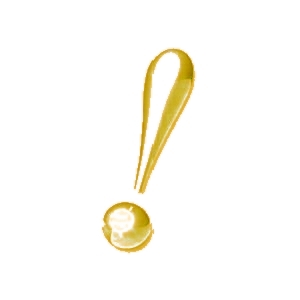
\includegraphics[scale=.25]{Graph/exclamation-mark}
	\end{flushright}
	\begin{block}{calculation of moments}
		\centering
		(central) moments (mean, power, variance, etc.) can be computed from 
		\begin{itemize}
			\item	the signal
			\item	the signal's PDF 
		\end{itemize}		
	\end{block}
\end{frame}		

\begin{frame}{audio signal description}{central moments summary}
\begin{footnotesize}
 \begin{table}
     \centering
         \begin{tabular}{lccccc}
             order & name & obs (cont) & pdf (cont) & \\\hline
            1 & $\mu_X$ & $\frac{1}{T}\int\limits_{-\nicefrac{T}{2}}^{\nicefrac{T}{2}} x(t)dt$ & $\int\limits_{-\infty}^{\infty}{xp_X(x)dx}$  \\
            2 & $\sigma_X^2$ & $\frac{1}{T}\int\limits_{-\nicefrac{T}{2}}^{\nicefrac{T}{2}}(x(t)-\mu_X)^2dt$ & $\int\limits_{-\infty}^{\infty} (x-\mu_X)^2p_X(x)dx$  \\
            %3 & skewness $\gamma_{X,3}$ & & $\int\limits_{-\infty}^{\infty} (x-\mu)^2p_X(x)dx$ &&\\
            %4 & kurtosis $\gamma_{X,4} & & $\int\limits_{-\infty}^{\infty} xp_X(x)dx$ &&\\
         \end{tabular}
 \end{table}
 \begin{table}
     \centering
         \begin{tabular}{lccccc}
             order & name  & obs (disc) & pdf (disc)\\\hline
            1 & $\mu_X$         &  $\frac{1}{N}\sum\limits_{i=0}^{N} x(i)$              & $\sum\limits_{\forall x} x p(x)$ \\
            2 & $\sigma_X^2$    &  $\frac{1}{N}\sum\limits_{i=0}^{N} (x(i)-\mu_X)^2$    & $\sum\limits_{\forall x} (x-\mu_X)^2p(x)$ \\
            %3 & skewness $\gamma_{X,3}$ & & $\int\limits_{-\infty}^{\infty} (x-\mu)^2p_X(x)dx$ &&\\
            %4 & kurtosis $\gamma_{X,4} & & $\int\limits_{-\infty}^{\infty} xp_X(x)dx$ &&\\
         \end{tabular}
 \end{table}
\end{footnotesize}
    \begin{itemize}
        \item[] standard deviation $\sigma_X = \sqrt{\sigma_X^2}$
    \end{itemize}
\end{frame}		

